\documentclass[zihao=-4,fontset = none]{ctexart}
\usepackage{xeCJKfntef}
\newif\ifpad

% \usepackage[paperwidth=10cm,paperheight=16cm,textwidth=240bp,vmargin=0.25cm]{geometry}
% \pagestyle{empty}

% \usepackage[a4paper,textwidth=492bp,vmargin=2cm]{geometry}
\usepackage{mwe}
\usepackage{amssymb,amsmath,amsthm}
\usepackage{unicode-math}
\allowdisplaybreaks[4]
\usepackage{siunitx,physics}
\sisetup{inter-unit-product = \ensuremath { { } \cdot { } } }
\theoremstyle{definition}
\newtheorem*{solution}{解}
\usepackage{xpatch}
\makeatletter
\xpatchcmd{\@thm}{\thm@headpunct{.}}{\thm@headpunct{:}}{}{}
\makeatother

% \setmainfont{Fira Sans}
% \setmathfont{Fira Math}

% \setmainfont{XITS}
% \setmathfont{XITS Math}
\xeCJKsetup{PunctStyle=kaiming}
% \setCJKmainfont[Mapping=fullwidth-stop]{Source Han Sans CN}

% \setCJKmainfont{Source Han Serif CN}[
%   UprightFont    = *-Regular,
%   BoldFont       = *-Bold,
%   ItalicFont     = 方正新楷体简体,
%   BoldItalicFont = *-Bold,
%   Mapping=fullwidth-stop
% ]
% \padtrue
\ifpad
\usepackage[paperwidth=10cm,paperheight=16cm,textwidth=20\ccwd,vmargin=0.5cm]{geometry}
\setmainfont{Fira Sans}
\setmathfont{Fira Math}
\setCJKmainfont[Mapping=fullwidth-stop]{Source Han Sans CN}
\usepackage{tikz,pgf}
\usetikzlibrary{shapes,calc}
\makeatletter
\newcommand\thumb{%
  \begingroup
  \tikzpicture[remember picture,overlay]
      \node[fill=gray,text=black,anchor=north east,xshift=0.15mm,
            yshift=-2.8mm,
            shape=semicircle,shape border rotate=90,
            minimum height=5mm,minimum width=2.5mm,
            font=\tiny\bfseries]
        at (current page.north east)
        {\arabic{page}\hspace*{-0.5\ccwd}};
  \endtikzpicture
  \endgroup
  }
\makeatother
\setlength{\headheight}{15pt}
\usepackage{fancyhdr}
\pagestyle{fancy}
\fancyhf{}
\fancyhead[r]{\thumb}
\renewcommand{\headrulewidth}{0pt}
\renewcommand{\footrulewidth}{0pt}
\else
\usepackage[a4paper,textwidth=41\ccwd,vmargin=2cm]{geometry}
\setmainfont{XITS}
\setmathfont{XITS Math}
\setCJKmainfont{Source Han Serif CN}[
  UprightFont    = *-Regular,
  BoldFont       = *-Bold,
  ItalicFont     = 方正新楷体简体,
  BoldItalicFont = *-Bold,
  Mapping=fullwidth-stop
]
\fi
\RequirePackage{enumitem,calc}
\setlist[enumerate,1]{leftmargin=0pt,labelsep=0pt,itemindent=0pt,parsep=5pt,itemsep=0pt,topsep=0pt,partopsep=0pt,listparindent=2\ccwd}
\setlist[enumerate,2]{leftmargin=0pt,labelsep=0pt,itemindent=1\ccwd+0.15cm,parsep=5pt,itemsep=0pt,topsep=0pt,partopsep=0pt,listparindent=2\ccwd}
\setlist[enumerate,3]{leftmargin=0pt,labelsep=0pt,itemindent=2\ccwd,parsep=5pt,itemsep=0pt,topsep=0pt,partopsep=0pt,listparindent=2\ccwd}
\def\labelenumi{\theenumi、}
\renewcommand{\theenumii}{\arabic{enumii}}
\def\labelenumii{(\theenumii)}
\renewcommand{\theenumiii}{\alph{enumiii}}

\setlength{\lineskip}{2.5pt}
\setlength{\lineskiplimit}{2.5pt}

\usepackage[hidelinks,bookmarks=true,bookmarksopen=true,bookmarksnumbered=true]{hyperref}

\makeatletter
\def\@maketitle{%
  \newpage
  \null
  \vskip 2em%
  \begin{center}%
  \let \footnote \thanks
    {\LARGE \@title \par}%
  \end{center}%
  \par
  \vskip 1.5em}
\makeatother

\def\ee{\mathrm{e}}
\def\xiahua#1{\CJKunderline*[thickness=0.75pt]{#1}}



\title{《高电压技术》复习题}
\begin{document}
\maketitle
\tableofcontents
\section{作业题}
\begin{enumerate}
  \item 气体放电过程中产生带电质点最重要的方式是什么?为什么?
  \begin{solution}
    碰撞电离是气体放电过程中产生带电质点最重要的方式。

    这是因为电子体积小,其自由行程比离子大得多,所以在电场中获得的动能比离子大得多。
    
    其次,由于电子的质量远小于原子或分子,因此当电子的动能不足以使中性质点电离时,电子会遭到弹射而几乎不损失其动能;而离子因其质量与被撞的中性质点相近,每次碰撞都会使其速度小,影响其动能的积累。
  \end{solution}
  \item 简述汤逊放电理论。
  \begin{solution}
    设外界光电离因素在阴极表面产生了一个自由电子,此电子到达阳极表面时由于 $\alpha$ 过程,电子总数增至 $\ee^{αd}$ 个。因在对 $\alpha$ 系数进行讨论时已假设每次电离撞出一个正离子,故电极空间共有 $(\ee^{αd}-1)$ 个正离子。按照系数 $\gamma$ 的定义,此 $(\ee^{αd}-1)$ 个正离子在到达阴极表面时可撞出 $\gamma(\ee^{αd}-1)$ 个新电子,这些电子在电极空间的碰撞电离同样又能产生更多的正离子,如此循环下去。汤逊理论的自持放电条件可表达为 $\gamma(\ee^{αd}-1)=1$。
    % 当外施电压足够高时,一个电子从阴极出发向阳极运动,由于碰撞游离形成电子崩,则到达阳极并进入阳极的电子数为 $\ee^{αd}$ 个($α$为一个电子在电场作用下移动单位行程所发生的碰撞游离数;$d$ 为间隙距离)。因碰撞游离而产生的新的电子数或正离子数为 $(\ee^{αd}-1)$ 个。这些正离子在电场作用下向阴极运动,并撞击阴极.若 1 个正离子撞击阴极能从阴极表面释放 $\gamma$ 个($\gamma$为正离子的表面游离系数)有效电子,则 $(\ee^{αd}-1)$ 个正离子撞击阴极表面时可撞出 $\gamma(\ee^{αd}-1)$ 个新电子,则放电达到自持放电。即汤逊理论的自持放电条件可表达为 $\gamma(\ee^{αd}-1)=1$。
  \end{solution}
  \item 为什么棒—板间隙中棒为正极性时电晕起始电压比负极性时略高。
  \begin{solution}
    \begin{enumerate}
      \item 当棒具有正极性时,间隙中出现的电子向棒运动,进入强电场区,开始引起电离现象而形成电子崩。随着电压的逐渐上升,到放电达到自持、爆发电晕之前,在间隙中形成相当多的电子崩。当电子崩达到棒极后,其中的电子就进入棒极,而正离子仍留在空间,相对来说缓慢地向板极移动。于是在棒极附近,积聚起正空间电荷,从而减少了紧贴棒极附近的电场,而略为加强了外部空间的电场。这样,棒极附近的电场被削弱,难以造成流柱,这就使得自持放电也即电晕放电难以形成。 
      \item 当棒具有负极性时,阴极表面形成的电子立即进入强电场区,造成电子崩。当电子崩中的电子离开强电场区后,电子就不再能引起电离,而以越来越慢的速度向阳极运动。一部份电子直接消失于阳极,其余的可为氧原子所吸附形成负离子。电子崩中的正离子逐渐向棒极运动而消失于棒极,但由于其运动速度较慢,所以在棒极附近总是存在着正空间电荷。结果在棒极附近出现了比较集中的正空间电荷,而在其后则是非常分散的负空间电荷。负空间电荷由于浓度小,对外电场的影响不大,而正空间电荷将使电场畸变。棒极附近的电场得到增强,因而自持放电条件易于得到满足、易于转入流柱而形成电晕放电。
    \end{enumerate}
  \end{solution}
  \item \label{ti:4}雷电冲击电压的标准波形的波前和波长时间是如何确定的?
  \begin{solution}
    图~\ref{fig:4} 表示雷电冲击电压的标准波形和确定其波前和波长时间的方法(波长指冲击波衰减至半峰值的时间)。图中 $O$ 为原点,$P$ 点为波峰。国际上都用图示的方法求得名义零点 $O_1$。图中虚线所示,连接 $P$ 点与 $0.3$ 倍峰值点作虚线交横轴于 $O_1$ 点,这样波前时间 $T_1$、和波长 $T_2$ 都从 $O_1$ 算起。
    \begin{figure}[htbp]
      \centering
      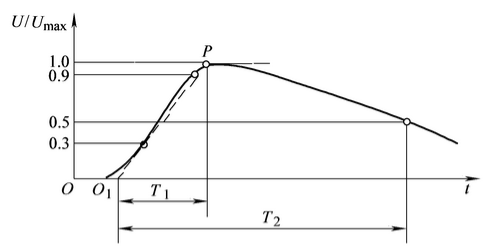
\includegraphics[width=0.5\textwidth]{3.png}
      \caption{第~\ref{ti:4} 题的图}\label{fig:4}
    \end{figure}
  \end{solution}
  \item 操作冲击放电电压的特点是什么?
  \begin{solution}
    \begin{enumerate}
      \item $U$ 形曲线,其击穿电压与波前时间有关而与波尾时间无关;
      \item 极性效应,正极性操作冲击的 \SI{50}{\percent} 击穿电压都比负极性的低;
      \item 饱和现象;
      \item 分散性大;
      \item 邻近效应,接地物体靠近放电间隙会显著降低正极性击穿电压。
    \end{enumerate}
  \end{solution}
  \item 影响套管沿面闪络电压的主要因素有哪些?
  \begin{solution}
    \begin{enumerate}
      \item 电场分布情况和作用电压波形的影响;
      \item 电介质材料的影响;
      \item 气体条件的影响;
      \item 雨水的影响。
    \end{enumerate}
  \end{solution}
  \item 具有强垂直分量时的沿面放电和具有弱垂直分量时的沿面放电,哪个对于绝缘的危害比较大,为什么?
  \begin{solution}
    具有强垂直分量时的沿面放电对绝缘的危害比较大。电场具有弱垂直分量的情况下,电极形状和布置已使电场很不均匀,因而介质表面积聚电荷使电压重新分布所造成的电场畸变,不会显著降低沿面放电电压。另外这种情况下电场垂直分量较小。沿表面也没有较大的电容电流流过,放电过程中不会出现热电离现象,故没有明显的滑闪放电,因而垂直于放电发展方向的介质厚度对放电电压实际上没有影响。其沿面闪络电压与空气击穿电压的差别相比强垂直分量时要小得多。
  \end{solution}
  \item 某距离4m的棒-极间隙。在夏季某日干球温度 $=\SI{30}{\degreeCelsius}$,湿球温度 $=\SI{25}{\degreeCelsius}$,气压 $=\SI{99.8}{kPa}$ 的大气条件下,问其正极性 $\SI{50}{\percent}$ 操作冲击击穿电压为多少 \si{kV}?(空气相对密度 $=0.95$)
  \begin{solution}
    距离为 \SI{4}{m} 的棒—极间隙,其标准参考大气条件下的正极性 \SI{50}{\percent} 操作冲击击穿电压 $U = \SI{1300}{kV}$。
    
    可得空气绝对湿度 $h=\SI{20}{g/m^3}$。从而 $\frac{h}{\delta} = 21$,求得参数 $K=1.1$。求得参数 $g = \frac{U_b}{500L} \frac{1}{\delta K} = 0.62$,于是求得指数 $m = W = 0.34$。
    
    空气密度校正因数 $K_d = \delta^m = 0.95^{0.34} = 0.9827$。
    
    湿度校正因数 $K_h = K^w = 1.1^{0.34} = 1.033$。
    
    冲击击穿电压 $U_{50\text{ 夏}} = U \cdot K_1 \cdot K_2 = 1300 \times 0.9827 \times 1.033 = \SI{1320}{kV}$。
  \end{solution}
  \item 某母线支柱绝缘子拟用于海拔 \SI{4500}{m} 的高原地区的 \SI{35}{kV} 变电站,问平原地区的制造厂在标准参考大气条件下进行 \SI{1}{min} 工频耐受电压试验时,其试验电压应为多少 \si{kV}?
  \begin{solution}
    \SI{35}{kV} 母线支柱绝缘子的 \SI{1}{min} 干工频耐受电压应为 \SI{100}{kV},则
    \[ U = \frac{U}{1.1 - 10^{-4}H} = \frac{100}{1.1 - 4500 \times 10^{-4}} = \SI{154}{kV} \]
  \end{solution}
  \item 什么叫电介质的极化?极化强度是怎么定义的?
  \begin{solution}
    电介质的极化是电介质在电场作用下,其束缚电荷相应于电场方向产生弹性位移现象和偶极子的取向现象。电介质的极化强度可用介电常数的大小来表示,它与该介质分子的极性强弱有关,还受到温度、外加电场频率等因素的影响。
  \end{solution}
  \item 固体无机电介质中,无机晶体、无机玻璃和陶瓷介质的损耗主要由那些损耗组成?
  \begin{solution}
    \begin{enumerate}
      \item 无机晶体介质只有位移极化,其介质损耗主要来源于电导;
      \item 无机玻璃的介质损耗可以认为主要由三部分组成:电导损耗、松弛损耗和结构损耗;
      \item 陶瓷介质可分为含有玻璃相和几乎不含玻璃相两类,第一类陶瓷是含有大量玻璃相和少量微晶的结构,其介质损耗主要由三部分组成:玻璃相中离子电导损耗、结构较松的多晶点阵结构引起的松弛损耗以及气隙中含水引起的界面附加损耗,$\tan \delta$ 相当大。第二类是由大量的微晶晶粒所组成,仅含有极少量或不含玻璃相,通常结晶相结构紧密,$\tan \delta$ 比第一类陶瓷小得多。
    \end{enumerate}
  \end{solution}
  \item 固体介质的表面电导率除了介质的性质之外,还与那些因素有关?它们各有什么影响?
  \begin{solution}
    介质的表面电导率 $\gamma_s$,不仅与介质的性质有关,而且强烈地受到周围环境的湿度、温度、表面的结构和形状以及表面粘污情况的影响。
    \begin{enumerate}
      \item 电介质表面吸附的水膜对表面电导率的影响
      
      由于湿空气中的水分子被吸附于介质的表面,形成一层很薄的水膜。因为水本身为半导体($\rho_v=\SI{e5}{\ohm m}$),所以介质表面的水膜将引起较大的表面电流,使 $\gamma_s$ 增加。
      \item 电介质的分子结构对表面电导率的影响
      
      电介质按水在介质表面分布状态的不同,可分为亲水电介质和疏水电介质两大类。
      \begin{enumerate}
        \item 亲水电介质:这种介质表面所吸附的水易于形成连续水膜,故表面电导率大,特别是一些含有碱金属离子的介质,介质中的碱金属离子还会进入水膜,降低水的电阻率,使表面电导率进一步上升,甚至丧失其绝缘性能。
        \item 疏水电介质:这些介质分子为非极性分子所组成,它们对水的吸引力小于水分子的内聚力,所以吸附在这类介质表面的水往往成为孤立的水滴,其接触角 $θ>90^\circ$,不能形成连续的水膜,故 $\gamma_s$ 很小,且大气湿度的影响较小。
      \end{enumerate}
      \item 电介质表面清洁度对表面电导率的影响
      
      表面沾污特别是含有电解质的沾污,将会引起介质表面导电水膜的电阻率下降,从而使 $\gamma_s$ 升高。
    \end{enumerate}
  \end{solution}
  \item 局部放电引起电介质劣化、损伤的主要原因有那些?
  \begin{solution}
    局部放电引起电介质劣化损伤的机理是多方面的,但主要有如下三个方面:
    \begin{enumerate}
      \item 电的作用:带电粒子对电介质表面的直接轰击作用,使有机电介质的分子主链断裂;
      \item 热的作用:带电粒子的轰击作用引起电介质局部的温度上升,发生热熔解或热降解;
      \item 化学作用:局部放电产生的受激分子或二次生成物的作用,使电介质受到的侵蚀可能比电、热作用的危害更大。
    \end{enumerate}
  \end{solution}
  \item 均匀固体介质的热击穿电压是如何确定的?
  \begin{solution}
    一般情况下,可以近似化为以下两种极端情况来讨论
    \begin{enumerate}
      \item 脉冲热击穿
      
      认为电场作用时间很短,以致导热过程可以忽略不计,则热平衡方程为
      \( c_v \frac{\dd{T}}{\dd{t}} = \gamma E^2 \)。
      \item 稳态热击穿
      
      电压长时间作用,介质内温度变化极慢,热击穿临界电压为
      \( U_{OC}^2 = 8 \int_{T_0}^T \frac{K}{\gamma} \dd{T} \)。
    \end{enumerate}
  \end{solution}
  \item 试比较气体、液体和固体介质击穿过程的异同。
  \begin{solution}
    \begin{enumerate}
      \item 气体介质的击穿过程
      
      气体放电都有从电子碰撞电离开始发展到电子崩的阶段。

      由于外电离因素的作用,在阴极附近出现一个初始电子,这一电子在向阳极运动时,如电场强度足够大,则会发生碰撞电离,产生 1 个新电子。新电子与初始电子在向阳极的行进过程中还会发生碰撞电离,产生两个新电子,电子总数增加到 4 个。第三次电离后电子数将增至 8 个,即按几何级数不断增加。电子数如雪崩式的增长,即出现电子崩。
      \item 液体介质的击穿过程
      \begin{enumerate}
        \item 电击穿理论以碰撞电离开始为击穿条件。
        
        液体介质中由于阴极的场致发射或热发射的电子在电场中被加速而获得动能,在它碰撞液体分子时又把能量传递给液体分子,电子损失的能量都用于激发液体分子的热振动。当电子在相邻两次碰撞间从电场中得到的能量大于 $\hbar v$ 时,电子就能在运动过程中逐渐积累能量,至电子能量大到一定值时,电子与液体相互作用时便导致碰撞电离。
        \item 气泡击穿理论
        
        液体中存在气泡时,由于交变电压下两串联介质中电场强度与介质介电常数成反比,气泡中的电场强度比液体介质高,而气体的击穿场强又比液体介质低得多,所以气泡先发生电离,使气泡温度升高,体积膨胀,电离进一步发展;而气泡电离产生的高能电子又碰撞液体分子,使液体分子电离生成更多的气体,扩大气体通道,当气泡在两极间形成“气桥”时,液体介质就能在此通道中发生击穿。
      \end{enumerate}
      \item 固体介质的击穿过程
      
      固体电介质的击穿中,常见的有热击穿、电击穿和不均匀介质局部放电引起击穿等形式。
      \begin{enumerate}
        \item 热击穿
        
        当固体电介质加上电场时,电介质中发生的损耗将引起发热,使介质温度升高,最终导致热击穿。
        \item 电击穿
        
        在较低温度下,采用了消除边缘效应的电极装置等严格控制的条件下,进行击穿试验时出现的一种击穿现象。
        \item 不均匀介质局部放电引起击穿
        
        从耐电强度低的气体开始,表现为局部放电,然后或快或慢地随时间发展至固体介质劣化损伤逐步扩大,致使介质击穿。
      \end{enumerate}
    \end{enumerate}
  \end{solution}
  \item 电介质极化的基本形式有哪几种,各有什么特点?
  \begin{solution}
    \begin{enumerate}
      \item 电子位移极化;
      \item 偶极子极化;
      \item 离子式极化;
      \item 夹层极化;
      \item 空间电荷极化。
    \end{enumerate}
  \end{solution}
  \item 如何用电介质极化的微观参数去表征宏观现象?
  \begin{solution}
    克劳休斯方程表明,要由电介质的微观参数($N$、$\alpha$)求得宏观参数一介电常数 $\varepsilon_r$,必须先求得电介质的有效电场 $E_i$。
    \begin{enumerate}
      \item 对于非极性和弱极性液体介质,有效电场强度
      \[ E_i = E + \frac{P}{3\varepsilon_0} = \frac{\varepsilon_r + 2}{3} E \]
      式中,$P$ 为极化强度。上式称为莫索缔(Mosotti)有效电场强度,将其代入克劳休斯方程,得到非极性与弱极性液体介质的极化方程为
      \[ \frac{\varepsilon_r - 1}{\varepsilon_r + 2} = \frac{N \alpha}{3 \varepsilon_0} \]
      \item 对于极性液体介质,由于极性液体分子具有固有偶极矩,它们之间的距离近,相互作用强,造成强的附加电场,洛伦兹球内分子作用的电场 $E_2 \ne 0$,莫索缔有效电场不适用。
    \end{enumerate}
  \end{solution}
  \item 极性液体的介电常数与温度、电压、频率有什么样的关系?
  \begin{solution}
    \begin{enumerate}
      \item 温度对极性液体电介质的 $\varepsilon_r$ 值的影响
      
      如图2-2所示,当温度很低时,由于分子间的联系紧密,液体电介质黏度很大,偶极子转动困难,所以 $\varepsilon_r$ 很小;随着温度的升高,液体电介质黏度减小,偶极子转动幅度变大,$\varepsilon_r$ 随之变大;温度继续升高,分子热运动加剧,阻碍极性分子沿电场取向,使极化减弱,$\varepsilon_r$ 又开始减小。
      \item 频率对极性液体电介质的 $\varepsilon_r$ 值的影响
      
      如图2-1所示,频率太高时偶极子来不及转动,因而 $\varepsilon_r$ 值变小。其中 $\varepsilon_{r0}$ 相当于直流电场下的介电常数,$f>f_1$ 以后偶极子越来越跟不上电场的交变,$\varepsilon_r$ 值不断下降;当频率 $f=f_2$ 时,偶极子已经完全跟不上电场转动了,这时只存在电子式极化,$\varepsilon_r$ 减小到 $\varepsilon_{r\infty}$,常温下,极性液体电介质的 $\varepsilon \approx 3 \sim 6$。
    \end{enumerate}
  \end{solution}
  \item 测量绝缘电阻能发现哪些绝缘缺陷?试比较它与测量泄漏电流试验项目的异同。
  \begin{solution}
    测量绝缘电阻能有效地发现下列缺陷:总体绝缘质量欠佳;绝缘受潮;两极间有贯穿性的导电通道;绝缘表面情况不良。测量绝缘电阻和测量泄露电流试验项目的相同点:两者的原理和适用范围是一样的,不同的是测量泄漏电流可使用较高的电压(\SI{10}{kV} 及以上),因此能比测量绝缘电阻更有效地发现一些尚未完全贯通的集中性缺陷。
  \end{solution}
  \item 绝缘干燥时和受潮后的吸收特性有什么不同?为什么测量吸收比能较好的判断绝缘是否受潮?
  \begin{solution}
    绝缘干燥时的吸收特性 $\frac{R_\infty}{R_0} > 2$,而受潮后的吸收特性 $\frac{R_\infty}{R_0} \approx 1$。如果测试品受潮,那么在测试时,吸收电流不仅在起始时就减少,同时衰减也非常快,吸收比的比值会有明显不同,所以通过测量吸收比可以判断绝缘是否受潮。
  \end{solution}
  \item 总结进行各种预防性试验时应注意的事项。
  \begin{solution}
    测量绝缘电阻时应注意下列几点:
    \begin{enumerate}
      \item 试验前应将试品接地放电一定时间。对容量较大的试品,一般要求 5--\SI{10}{min}。这是为了避免被试品上可能存留残余电荷而造成测量误差。试验后也应这样做,以求安全。
      \item 高压测试连接线应尽量保持架空,确需使用支撑时,要确认支撑物的绝缘对被试品绝缘测量结果的影响极小。
      \item 测量吸收比时,应待电源电压达稳定后再接入试品,并开始计时。
      \item 对带有绕组的被试品,加先将被测绕组首尾短接,再接到 L 端子:其他非被测绕组也应先首尾短接后再接到应接端子。
      \item 绝缘电阻与温度有十分显著的关系。绝缘温度升高时,绝缘电阻大致按指数率降低。吸收比的值也会有所改变。所以,测量绝缘电阻时,应准确记录当时绝缘的温度,而在比较时,也应按相应温度时的值来比较。
      \item 每次测试结束时,应在保持兆欧表电源电压的条件下,先断开 L 端子与被试品的连线,以免试品对兆欧表反向放电,损坏仪表。
    \end{enumerate}
  \end{solution}
  \item 综合讨论:现行对绝缘的离线检查性试验存在哪些不足之处?探索一下:对某些电气设备绝缘进行在线检测的可能性和原理性方法。
  \begin{solution}
    不足之处:需要停电进行,而不少重要的电力设备不能轻易地停止运行;监测间隔周期较长,不能及时发现绝缘故障;停电后的设备状态与运行时的设备状态不相符,影响诊断的正确性。
  \end{solution}
\end{enumerate}

\section{复习题(一)}
\subsection{填空题}
\begin{enumerate}
  \item 处于电场中的绝缘电介质,必然会存在一定的能量损耗,这些由极化、电导等因素引起的损耗称为\xiahua{介质损耗},其主要来源于\xiahua{电导损耗}和\xiahua{松弛损耗}两个方面。
  \item 汤逊理论认为:\xiahua{碰撞电离}是气体放电时电流倍增的主要过程,而\xiahua{阴极表面的电子发射}是维持放电的重要条件。
  \item 电介质的极化强弱可用\xiahua{介电常数}的大小来表示。它与该介质分子的极性强弱有关,还受到\xiahua{温度}、\xiahua{外加电场频率}等因素的影响。
  \item 直流电压下电介质仅有\xiahua{电导}所引起的损耗;交流电压下电介质既有\xiahua{电导}损耗,又有\xiahua{极化}损耗。
  \item 大型高电压试验设备通常包括\xiahua{工频高电压试验设备},\xiahua{直流高电压发生器}和\xiahua{冲击电压发生器}。
  \item 在对电力设备绝缘进行高电压耐压试验时,所采用的电压波形有\xiahua{直流}、\xiahua{交流}、\xiahua{雷电过电压}、\xiahua{操作冲击波}。
  \item 在局部放电测量中,$\Delta q$ 称为\xiahua{视在放电量}。
  \item 纯净液体介质的击穿理论分为\xiahua{电击穿理论}和\xiahua{气泡击穿理论}。
\end{enumerate}

\subsection{简答题}
\begin{enumerate}
  \item 为什么棒—板间隙中棒为正极性时电晕起始电压比负极性时略高?
  \begin{solution}
    \begin{enumerate}
      \item 当棒具有正极性时,间隙中出现的电子向棒运动,进入强电场区,开始引起电离现象而形成电子崩。随着电压的逐渐上升,到放电达到自持、爆发电晕之前,在间隙中形成相当多的电子崩。当电子崩达到棒极后,其中的电子就进入棒极,而正离子仍留在空间,相对来说缓慢地向板极移动。于是在棒极附近,积聚起正空间电荷,从而减少了紧贴棒极附近的电场,而略为加强了外部空间的电场。这样,棒极附近的电场被削弱,难以造成流柱,这就使得自持放电也即电晕放电难以形成。 
      \item 当棒具有负极性时,阴极表面形成的电子立即进入强电场区,造成电子崩。当电子崩中的电子离开强电场区后,电子就不再能引起电离,而以越来越慢的速度向阳极运动。一部份电子直接消失于阳极,其余的可为氧原子所吸附形成负离子。电子崩中的正离子逐渐向棒极运动而消失于棒极,但由于其运动速度较慢,所以在棒极附近总是存在着正空间电荷。结果在棒极附近出现了比较集中的正空间电荷,而在其后则是非常分散的负空间电荷。负空间电荷由于浓度小,对外电场的影响不大,而正空间电荷将使电场畸变。棒极附近的电场得到增强,因而自持放电条件易于得到满足、易于转入流柱而形成电晕放电。
    \end{enumerate}
  \end{solution}
  \item 保护设备与被保护设备的伏秒特性应如何配合?为什么?
  \begin{solution}
    保护设备的伏秒特性应始终低于被保护设备的伏秒特性。这样,
    当有一过电压作用于两设备时,总是保护设备先击穿,进而限制了过
    电压幅值,保护了被保护设备。
  \end{solution}
  \item 正接法和反接法西林电桥各应用在什么条件下?
  \begin{solution}
    正接法一般应用于实验室内的测试材料及小设备,实现样品的对
    地绝缘。实际上, 绝大多数电气设备的金属外壳是直接放在接地底
    座上的,换句话说,就是试品的一极是固定接地的,这时就要用反接
    法。
  \end{solution}
  \item 对两类冲击波,中国和IEC标准怎么规定的?
  \begin{solution}
    第一类波形,中国和 IEC 标准规定了 4 种该类冲击波,即 \SI{1}{μs}/\SI{20}{μs},\SI{4}{μs}/\SI{10}{μs},\SI{8}{μs}/\allowbreak\SI{20}{μs} 和 \SI{30}{μs}/\SI{80}{μs} 冲击电流波。第
    二类规定的冲击电流波形峰值持续时间规定为 \SI{500}{μs},\SI{1000}{μs},
    \SI{2000}{μs} 或者 \SI{2000}{μs} 与 \SI{3200}{μs} 之间。
  \end{solution}
  \item 测量绝缘材料的泄漏电流为什么用直流电压而不用交流电压?
  \begin{solution}
    因为直流电压作用下的介质损失仅有漏导损失,而交流作用下的介质损失不仅有漏导损失还有极化损失。所以在直流电压下,更容易
    测量出泄漏电流。
  \end{solution}
\end{enumerate}
\subsection{计算题}
\begin{enumerate}
  \item 某母线支柱绝缘子拟用于海拔 \SI{4500}{m} 的高原地区的 \SI{35}{kV} 变电站,问平原地区的制造厂在标准参考大气条件下进行 \SI{1}{min} 工频耐受电压试验时,其试验电压应为多少 \si{kV}?
  \begin{solution}
    查 GB311.1-1997 的规定可知,\SI{35}{kV} 母线支柱绝缘子的 \SI{1}{min} 工频
    耐受电压应为 \SI{100}{kV},则可算出制造厂在平原地区进行出厂 \SI{1}{min} 工
    频耐受电压试验时,其耐受电压 $U$ 应为
    \[ U = \frac{U_0}{1.1-10^{-4}H} = \frac{100}{1.1-4500\times 10^{-4}} = \SI{154}{kV} \]
  \end{solution}
  \item 某 \SI{110}{kV} 电气设备的外绝缘应有的工频耐受电压为 \SI{260}{kV}(有效值),若将该设备安装在海拔 \num{3000} 米的地方运行,问出厂时在海拔 \num{1000} 米条件下工频试验电压应增大到多少?
  \begin{solution}
    出厂时的试验电压
    \[ U = K_a U_s = \ee^{m(H-1000)/8150} U_s \]
    将 $H=3000$,$U_s=260$,$m=1$ 代入可求得:$U = \SI{332.314}{kV}$。
  \end{solution}
  \item 一台测工频高电压的电阻分压器,额定电压为 \SI{100}{kV}(有效值),阻值为 \SI{4}{M\ohm},对地杂散电容为 \SI{1000}{pF},求由杂散电容引起的峰值和相位测量误差,以及在额定测量电压下热耗的功率值。
  \begin{solution}
    幅值误差
    \begin{align*}
      A &\approx 1 - \frac{(\omega R_1 C_e)^2}{180} \\
        &= 1 - \frac{\bigl( 2 \times 3.14 \times 50 \times 4 \times 10^6 \times 10^{-9} \bigr)^2}{180} \\
        &= 0.9912
    \end{align*}
    相角误差
    \[ \theta \approx \arctan(\omega R_1 C_e / 6) = \SI{11.82}{\percent} \]
    热耗的功率值
    \[ P = U^2/R = (100\times 10^3)^2/(4\times 10^6) = \SI{2500}{\W} \]
  \end{solution}
  \item \label{ti:1-4}某线路连接如图~\ref{fig:1-4} 所示,架空线路波阻抗 $Z_1 = \SI{500}{\ohm}$,电缆线路波阻抗 $Z_2 = \SI{50}{\ohm}$,在电缆首端接有 $R = \SI{100}{\ohm}$ 的电阻,现有一幅值 $U = \SI{500}{kV}$ 的直角波从线路 1 传入,求
  \begin{enumerate}
    \item 侵入电缆 $Z_2$ 的电压波幅值;(3分)
    \item 架空线路 $Z_1$ 中的反射电压与反射电流幅值;(3分)
    \item 流过 $R$ 的电流值;(4分)
  \end{enumerate}
  \begin{figure}[htbp]
    \centering
    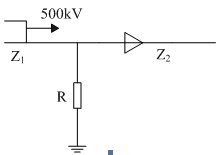
\includegraphics[width=0.5\textwidth]{1.png}
    \caption{第~\ref{ti:4} 题的图}\label{fig:1-4}
  \end{figure}
  \begin{solution}
    $Z_1 = \SI{500}{\ohm}$,$Z_2' = \frac{RZ_2}{R+Z_2} = \frac{50\times100}{50+100} = \frac{100}{3} = \SI{33.3}{\ohm}$。

    折射:$\alpha = \frac{2Z_2'}{Z_1 + Z_2'} = \frac{2 \frac{100}{3}}{500 + \frac{100}{3}} = \frac{1}{8} = 0.125$。

    反射:$\beta = \frac{Z_2' - Z_1}{Z_1 + Z_2'} = \frac{\frac{100}{3} - 500}{500 + \frac{100}{3}} = -\frac{7}{8} = -0.875$。
    \begin{enumerate}
      \item $U_{Z_2} = \alpha E = \frac{1}{8} \times 500 = \SI{62.5}{kV}$。
      \item $U_{1b} = \beta E = -\frac{7}{8} \times 500 = -\SI{437.5}{kV}$,
      $I_{1b} = -\frac{U_{1b}}{Z_1} = \SI{875}{A}$。
      \item $I_R = \frac{U_{Z_2}}{R} = \SI{625}{A}$。
    \end{enumerate}
  \end{solution}
\end{enumerate}

\section{复习题(二)}
\subsection{填空题}
\begin{enumerate}
  \item 影响液体电介质击穿电压的因素有\xiahua{杂质}、\xiahua{温度}、\xiahua{电场的均匀程度}、\xiahua{电压的作用时间}、\xiahua{压力}。
  \item 介质热老化的程度主要是由\xiahua{温度}和\xiahua{介质经受热作用时间}来决定的。
  \item 目前实用的局部放电测量的方法,使用得最多的测量方法是\xiahua{绝缘油的气相色谱分析}、\xiahua{超声波探测法}、\xiahua{脉冲电流法}。
  \item 在对电力设备绝缘进行高电压耐压试验时,所采用的电压波形有\xiahua{直流}、\xiahua{交流}、\xiahua{雷电过电压}、\xiahua{操作冲击波}。
  \item 交流高电压试验设备主要是指\xiahua{高电压试验变压器}。
  \item 试验变压器的体积和重量都随其额定电压值的增加而急剧增加,试验变压器的额定容量 $P_{\symup{n}}$ 应按\xiahua{被测试样在最不利的试验条件下需要的电流}来选择。
  \item 在对电力设备绝缘进行高电压耐压试验时,所采用的电压波形有\xiahua{直流}、\xiahua{交流}、\xiahua{雷电过电压}、\xiahua{操作冲击波}。
\end{enumerate}

\subsection{简答题}
\begin{enumerate}
  \item 叙述汤逊理论的基本观点和流注理论的基本观点以及它们的适用范围。
  \begin{solution}
    汤逊理论只适用于 $pd$ 值较小的范围,流注理论只适用于 $pd$ 值较
    大的范围,两者的过渡值为 $pd \approx \SI{26.66}{\kPa \cm}$。

    汤逊理论的基本观点是:电子的碰撞电离是气体放电时电流倍增的主要过程,而阴极表面的电子发射是维持放电的重要条件。

    流注理论的基本观点:
    \begin{enumerate}
      \item 以汤逊理论的碰撞电离为基础,强调空间电荷对电场的畸变作用,着重于用气体空间的光电离来解释气体放电通道的发展过程。
      \item 放电以起始到击穿并非碰撞电离连续量变的过程,当初始电子崩中
      离子数达到 \num{e8} 以上时,要引起空间光电离这样一个质的变化,此时
      由光子造成的二次崩向主崩汇合而形成流注。
      \item 流注一旦形成,放电就转入自持。
    \end{enumerate}
  \end{solution}
  \item 影响套管沿面闪络电压的主要因素有哪些?
  \begin{enumerate}
    \item 电场分布情况和作用电压波形的影响;
    \item 电介质材料的影响;
    \item 气体条件的影响;
    \item 雨水的影响。
  \end{enumerate}
  \item \label{ti:2-3}画出交流耐压试验接线图,说明各元件的作用。
  \begin{solution}
    % 交流耐压试验接线图见图~\ref{fig:2-3}。调压器 $\mathrm{T}_1$ 用来调节工频试验电压的大小和升降速度,试验变压器 $\mathrm{T}_2$ 用来升高电压供给被试品所需的高电压,球隙 G 是用来测量高电压(或保护被试品免受过电压),$R_1$ 用来限制被试品放电时试验变压器的短路电流不超过允许值和高压绕组的电压梯度不超过危险值,$R_2$ 用来限制球隙放电时的电流不致灼伤铜球表面。
    AV——调压器,PV1——低压侧电压表,T——工频高压装置,$R_1$——变压器保护电阻,TO——被测试品,$R_2$——测量球隙保护电阻,PV2——高压静电电压表,F——测量球隙,$L_{\mathrm{f}}$、$C_{\mathrm{f}}$——谐波滤波器。
    \begin{figure}[htbp]
      \centering
      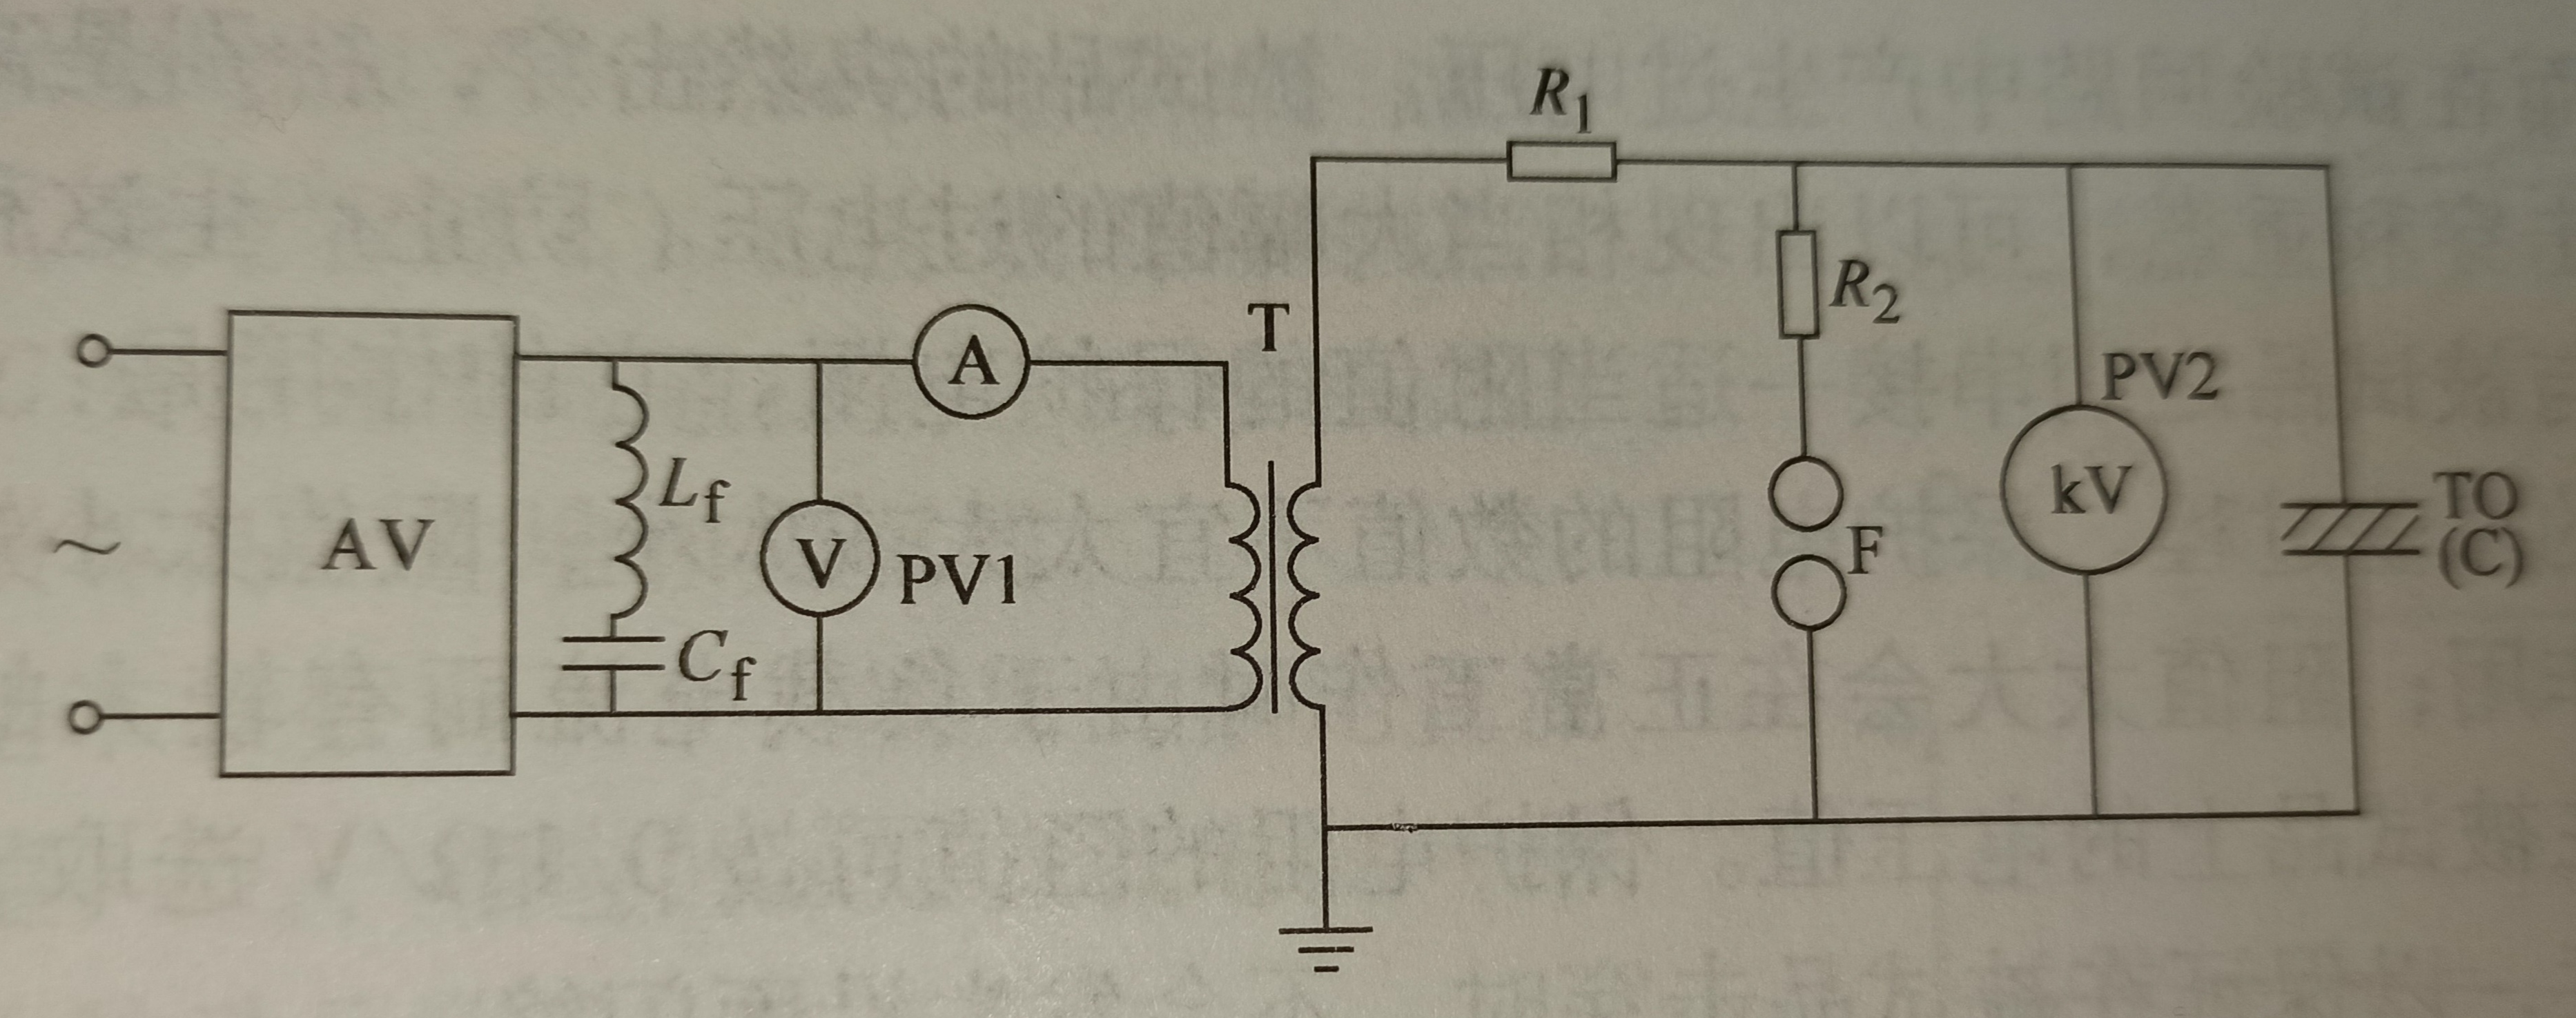
\includegraphics[width=\textwidth]{7.jpg}
      \caption{第~\ref{ti:2-3} 题的图}\label{fig:2-3}
    \end{figure}
  \end{solution}
  \item 测量绝缘材料的泄漏电流为什么用直流电压而不用交流电压?
  \begin{solution}
    因为直流电压作用下的介质损失仅有漏导损失,而交流作用下的介质损失不仅有漏导损失还有极化损失。所以在直流电压下,更容易
    测量出泄漏电流。
  \end{solution}
  \item 测量高电压的弱电仪器常受一些电磁干扰,干扰来源主要有哪些?
  \begin{solution}
    测量用的射频同轴电缆外皮中通过的瞬态电流引起的干扰,间隙
    放电时产生的空间电磁辐射,仪器电源线引入的干扰。
  \end{solution}
  \item 正接法和反接法西林电桥各应用在什么条件下?
  \begin{solution}
    正接法一般应用于实验室内的测试材料及小设备,实现样品的对
    地绝缘。实际上, 绝大多数电气设备的金属外壳是直接放在接地底
    座上的,换句话说,就是试品的一极是固定接地的,这时就要用反接
    法。
  \end{solution}
\end{enumerate}

\subsection{计算题}
\begin{enumerate}
  \item 一绝缘由两层电介质叠放构成,它们的介质损失角正切和电容分别为 $\tan δ_1$、$C_1$ 和 $\tan δ_2$、$C_2$,求串联介质总的介质损失角正切 $\tan δ$。
  \begin{solution}
    由 $\tan\delta_1 = \omega C_1R_1$,$\tan\delta_2 = \omega C_2R_2$,得 $R_1 = \frac{\tan\delta_1}{\omega C_1}$,$R_2 = \frac{\tan\delta_2}{\omega C_2}$。

    串联后:$R=R_1+R_2$,$C = \frac{C_1C_2}{C_1 + C_2}$。
    则
    \begin{align*}
      \tan\delta &= \omega CR = \omega \frac{C_1 C_2}{C_1+C_2} \Biggl( \frac{\tan\delta_1}{\omega C_1} + \frac{\tan\delta_2}{\omega C_2} \Biggr) \\
      &= \frac{ C_2 \tan\delta_1 + C_1 \tan\delta_2 }{C_1+C_2}
    \end{align*}
  \end{solution}
  \item 一固体电介质,其电容量 $C = \SI{2000}{pF}$;$\tan δ =\SI{1}{\percent}$;绝缘电阻 $R=\SI{2000}{MΩ}$,求:
  \begin{enumerate}
    \item 施加工频电压 $U=\SI{100}{kV}$(有效值),介质损耗为多少?
    \item 施加直流电压 $U=\SI{100}{kV}$,介质损耗为多少?
  \end{enumerate}
  \begin{solution}
    \begin{enumerate}
      \item 交流情况下:
      \begin{align*}
        p &= ui\cos\varphi = U^2 \omega C \tan\delta \\
          &= 100^2 \times 10^6 \times 2 \symup \pi \times 50 \times 2000 \times 10^{-12} \times \SI{1}{\percent} \\
          &= 20 \symup \pi = \SI{62.8}{W}
      \end{align*}
      \item 直流情况下:
      \[ p = \frac{U^2}{R} = \frac{(100 \times 10^3)^2}{2000 \times 10^6} = \SI{5}{W} \]
    \end{enumerate}
  \end{solution}
  \item \label{ti:2-7}某变电所母线接线图如图~\ref{fig:2-7} 所示,各路出线波阻抗 $Z=\SI{400}{Ω}$,现有一幅值 $U=\SI{500}{kV}$ 的无穷长直角波由其中一路出线侵入变电所,求变电所母线上电压幅值。
  \begin{figure}[htbp]
    \centering
    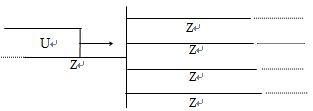
\includegraphics[width=0.5\textwidth]{2.png}
    \caption{第~\ref{ti:2-7} 题的图}\label{fig:2-7}
  \end{figure}
  \begin{solution}
    母线上电压:
    \[ U_B = 2 u \frac{z/4}{z+z/4} = 2u/5 = \SI{200}{kV} \]
    彼得逊等值电路如图~\ref{fig:2-7-2} 所示。
    \begin{figure}[htbp]
      \centering
      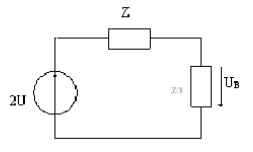
\includegraphics[width=0.5\textwidth]{5.png}
      \caption{彼得逊等值电路}\label{fig:2-7-2}
    \end{figure}
  \end{solution}
  \item 一台测工频高电压的电阻分压器,额定电压为 \SI{100}{kV}(有效值),阻值为 \SI{4}{MΩ},对地杂散电容为 \SI{1000}{pF},求由杂散电容引起的峰值和相位测量误差,以及在额定测量电压下热耗的功率值。
  \begin{solution}
    幅值误差
    \begin{align*}
      A &\approx 1 - \frac{(\omega R_1 C_e)^2}{180} \\
        &= 1 - \frac{\bigl( 2 \times 3.14 \times 50 \times 4 \times 10^6 \times 10^{-9} \bigr)^2}{180} \\
        &= 0.9912
    \end{align*}
    相角误差
    \[ \theta \approx \arctan(\omega R_1 C_e / 6) = \SI{11.82}{\percent} \]
    热耗的功率值
    \[ P = U^2/R = (100\times 10^3)^2/(4\times 10^6) = \SI{2500}{\W} \]
  \end{solution}
\end{enumerate}

\section{复习题(三)}
\subsection{填空题}
\begin{enumerate}
  \item 流注理论认为,碰撞游离和\xiahua{空间光电离}是形成自持放电的主要因素。
  \item 工程实际中,常用棒—板或\xiahua{棒—棒}电极结构研究极不均匀电场下的击穿特性。
  \item 气体中带电质子的消失有\xiahua{扩散}、复合、附着效应等几种形式。
  \item 我国国家标准规定的标准操作冲击波形成 \xiahua{250 / 2500} \si{\us}。
  \item 极不均匀电场中,屏障的作用是由于其对\xiahua{空间电荷}的阻挡作用,造成电场分布的改变。
  \item 下行的负极性雷通常可分为 3 个主要阶段:\xiahua{先导}、\xiahua{主放电}、\xiahua{余光}。
  \item 调整电场的方法:\xiahua{增大}电极曲率半径、改善电极边缘、使电极具有最佳外形。
  \item 介质损失角正切的计算公式是\xiahua{ $P/Q$(有功功率/无功功率)},$\tan\delta$ 表示\xiahua{介质损耗因数}。
  \item 一般来说,标准电容器采用\xiahua{气体}绝缘,电力电容器采用\xiahua{油纸}绝缘,为什么?
\end{enumerate}

\subsection{简答题}
\begin{enumerate}
  \item 对架空线路绝缘子串,如何确定工作电压其所需绝缘子片数?如何确定操作过电压下其所需绝缘子片数?
  \begin{solution}
    在根据杆塔机械载荷选定绝缘子型式之后,需要确定每串绝缘子的片数,以满足下列要求:
    \begin{enumerate}
      \item 在工作电压下不发生污闪;
      \item 雨天时在操作过电压作用下不发生闪络(湿闪);
      \item 具有一定的雷电冲击耐压强度,保证一定的线路耐雷水平。
    \end{enumerate}
    确定绝缘子串的片数的具体做法简介如下:
    \begin{enumerate}
      \item 按工作电压下所要求的泄漏距离(爬电比距)$s$ 决定所需绝缘子片
      数 $n$ 绝缘子串应有足够的沿面爬电比距以防止在工作电压下发生污
      闪。具体的作法是:按工作电压下所需求的泄漏距离决定所需绝缘子
      片数,然后按操作过电压及耐雷水平的要求进行验算。爬电比距定义
      如下:
      \[ s = \frac{n \lambda}{U} \si{\cm/\kV} \]
      式中\begin{tabular}[t]{r@{——}l}
        $n$ & 每串绝缘子的片数 \\
        $\lambda$ & 每片绝缘子的爬电距离,\si{cm} \\
        $U$ & 线路的额定电压(有效值),\si{kV}
      \end{tabular}

      对于不同的污秽地区要求一定的爬电比距 $S_0$,必须满足 $S \geqslant S_0$,否则污闪事故将比较严重,会造成很大损失。《高压电力设备外绝缘污
      秽等级》中把外绝缘按污染程度划分为 0、I、II、III、IV 级,其中 0
      级相应于无明显污秽地区。

      由此可得出根据最高工作线电压确定每串绝缘子的片数为
      \[ n_1 \geqslant \frac{S_0 U}{\lambda} \]
      \item 按内部过电压进行验算绝缘子串除应在长期工作电压下不发生闪
      络外,还应耐受操作过电压的作用。即绝缘子串的湿闪电压在考虑大
      气状态等影响因素并保持一定的裕度后,应大于可能出现的操作过电
      压。通常取 \SI{10}{\percent} 的裕度.则绝缘于的工频或操作湿闪电压 $U_{sh}$ 为
      \[ U_{sh} = 1.1 k_0 U_{xg} \]
      式中 $k_0$ 为操作过电压的计算倍数;$U_{xg}$ 为最高运行相电压。
    \end{enumerate}
  \end{solution}
  \item 叙述汤逊理论的基本观点和流注理论的基本观点以及它们的适用范围。
  \begin{solution}
    汤逊理论只适用于 $pd$ 值较小的范围,流注理论只适用于 $pd$ 值较
    大的范围,两者的过渡值为 $pd \approx \SI{26.66}{\kPa \cm}$。

    汤逊理论的基本观点是:电子的碰撞电离是气体放电时电流倍增的主要过程,而阴极表面的电子发射是维持放电的重要条件。

    流注理论的基本观点:
    \begin{enumerate}
      \item 以汤逊理论的碰撞电离为基础,强调空间电荷对电场的畸变作用,着重于用气体空间的光电离来解释气体放电通道的发展过程。
      \item 放电以起始到击穿并非碰撞电离连续量变的过程,当初始电子崩中
      离子数达到 \num{e8} 以上时,要引起空间光电离这样一个质的变化,此时
      由光子造成的二次崩向主崩汇合而形成流注。
      \item 流注一旦形成,放电就转入自持。
    \end{enumerate}
  \end{solution}
  \item 简述冲击电流发生器的基本原理。
  \begin{solution}
    冲击电压发生器原理图见图~\ref{fig:3-3}。由一组高压大电容量的电容器,先通过直流高压并联充电,充电
    时间为几十秒到几分;然后通过触发球隙的击穿,并联地对试品放电,
    从而在试品上流过冲击大电流。
    \begin{figure}[htbp]
      \centering
      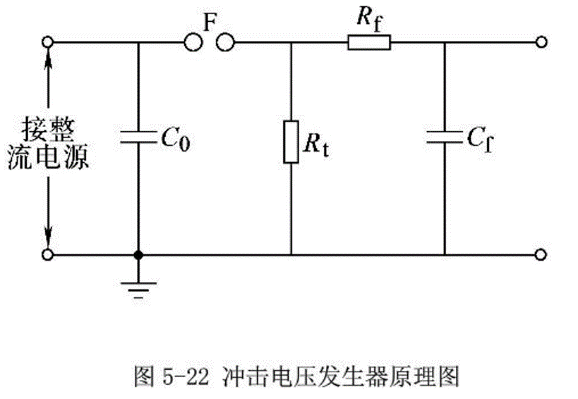
\includegraphics[width=0.5\textwidth]{6.png}
      \caption{冲击电压发生器原理图}\label{fig:3-3}
    \end{figure}
  \end{solution}
  \item 简述什么是在线检测,那些设备需要实施在线检测?在线检测与离线试验各有什么优缺点?
  \begin{solution}
    在线监测是在电力设备运行的状态下连续或周期性监测绝缘的状
    况。一些不能停止运行的重要电力设备需要实施在线监测。离线试验
    需要停电进行;监测间隔周期较长,不能及时发现绝缘故障;停电后的
    设备状态与运行时的设备状态不相符,影响诊断的正确性,但是离线
    试验投资较小;检测面宽;检测设备相对简单,使用方便;适合小型系
    统和设备,同时对设备的影响小。
  \end{solution}
\end{enumerate}

\subsection{计算题}
\begin{enumerate}
  \item 某母线支柱绝缘子拟用于海拔 \SI{4500}{m} 的高原地区的 \SI{35}{kV} 变电站,问平原地区的制造厂在标准参考大气条件下进行 \SI{1}{min} 工频耐受电压试验时,其试验电压应为多少 \si{kV}?
  \begin{solution}
    查 GB311.1-1997 的规定可知,\SI{35}{kV} 母线支柱绝缘子的 \SI{1}{min} 工频
    耐受电压应为 \SI{100}{kV},则可算出制造厂在平原地区进行出厂 \SI{1}{min} 工
    频耐受电压试验时,其耐受电压 $U$ 应为
    \[ U = \frac{U_0}{1.1-10^{-4}H} = \frac{100}{1.1-4500\times 10^{-4}} = \SI{154}{kV} \]
  \end{solution}
  \item 某 \SI{1000}{kV} 工频试验变压器,套管顶部为球形电极,球心距离四周墙壁均约 \SI{5}{m},问球电极直径至少要多大才能保证在标准参考大气条件下,当变压器升压到 \SI{1000}{kV} 额定电压时,球电极不发生电晕放电?
  \begin{solution}
    此球形电极与四周墙壁大致等距离,可按照上述的同心球电极结构来考虑。变压器的球电极为同心球的内电极,四周墙壁为同心球的外电极。

    按题意须保证点要求升压到 \SI{1000}{\kV}(有效值)时,球电极表面最大场强 $E_{\max}$ 小于球电极的电晕起始场强 $E_0$,即保证
    \[ \frac{RU}{r(R-r)} < 24 \delta \bigl( 1 + 1/\sqrt{r\delta} \bigr) \]
    将 $U=\SI{1414}{V}$ 峰值,$R=\SI{500}{\cm}$,$\delta = 1$ 代入此不等式,算得 $r=\SI{60}{cm}$ 时球电极表面最大场强 $E_{\max} = \SI{26.7}{\kV/\cm}$,小于同心球内电极的电晕起始场强 $E_0 = \SI{27.1}{\kV/\cm}$。球电极的起始电晕电压 $U_c = E_0 \frac{(R-r)r}{R} = \SI{1012}{kV} > \SI{1000}{kV}$。

    因此,在这种距离四周墙壁仅 \SI{5}{m} 的空间尺寸下,球电极的直径应达 \SI{120}{cm} 才能保证当变压器升压到 \SI{1000}{kV} 额定电压时球电极不发生电晕放电。
  \end{solution}
\end{enumerate}
\end{document}